\documentclass{article}
\usepackage{setspace}
\usepackage{tikz}
\usetikzlibrary{arrows}

\begin{document}

\doublespacing

\section{Phase I}
The behaviour of Phase I can be modelled as a finite state machine, as in the
diagram below.

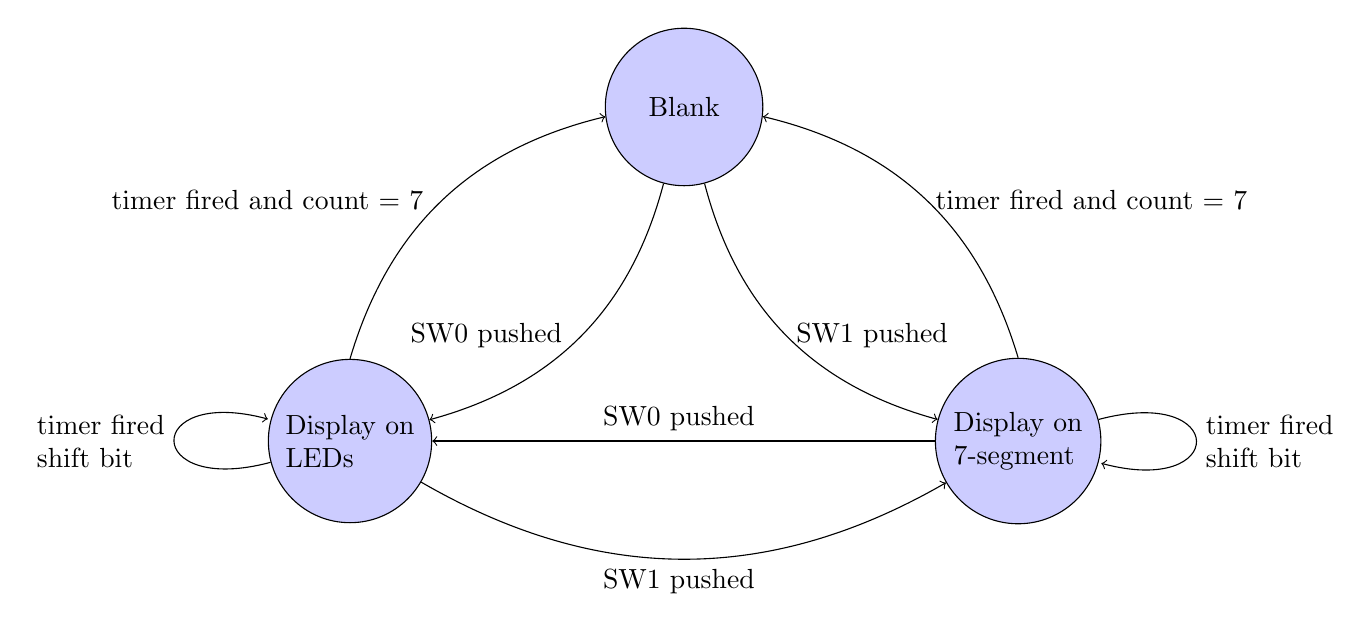
\begin{tikzpicture}[->,node distance=6cm,main/.style={circle,fill=blue!20,draw,minimum size=2cm,align=left}]
    \node[main] (blank) {Blank};
    \node[main] (led) [below left of=blank] {Display on\\LEDs};
    \node[main] (7seg) [below right of=blank] {Display on\\7-segment};
    \path[align=left]
        (blank) edge [bend left] node [left] { SW0 pushed } (led)
                edge [bend right] node [right] { SW1 pushed } (7seg)
        (led) edge [loop left] node { timer fired \\ shift bit } (led)
              edge [bend right] node [below] { SW1 pushed } (7seg)
        (led.north) edge [bend left] node [left] { timer fired and count = 7 } (blank)
        (7seg) edge [loop right] node { timer fired \\ shift bit } (7seg)
               edge node [above] { SW0 pushed } (led)
        (7seg.north) edge [bend right] node [right] { timer fired and count = 7 } (blank)
    ;
\end{tikzpicture}

\end{document}
